\chapter{Implementierung}
\label{chap:implementation}

Um die in Kapitel \ref{chap:threads} beschriebenen Probleme zu mindern oder gar zu beheben, kann eine Auswahl an vorgestellten Technologien (siehe \ref{chap:technologies}) genutzt werden. Das Ziel ist der Schutz einer kleinen Anzahl von Clients durch den Einsatz eines speziell konfigurierten, lokalen, rekursiven Resolvers. Es ist dabei nicht sinnvoll, alle anwendbaren Techniken einzusetzen, da jede mit Kosten in Performance einhergeht und die Vorteile mancher Kombinationen redundant sind.

\section{Position und Resolver Typ}
Die möglichen Positionen und Betriebsarten eines Resolvers (siehe Abb. \ref{img:impl-resolverpositions}) wurden bereits im Abschnitt \ref{sec:dnsresolverposition} behandelt. Für die Auswahl wurden drei Kriterien betrachtet: Angreifbarkeit, Performance und Privacy.
\begin{figure}[hb]
    \centering
    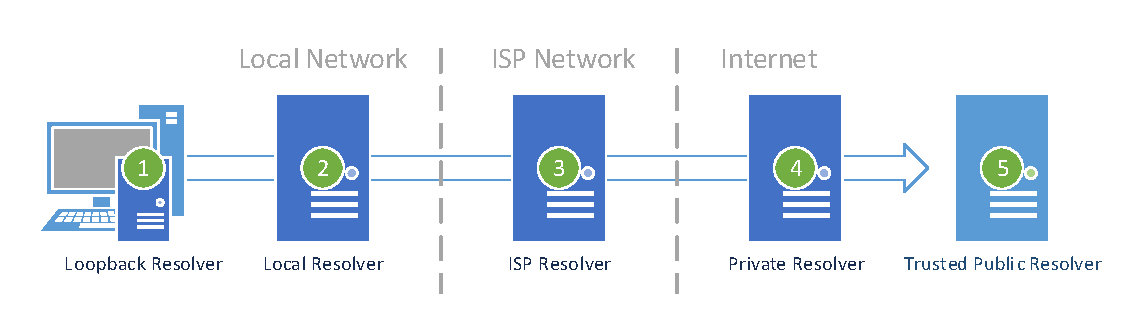
\includegraphics[width=\textwidth,trim={8mm 8mm 8mm 8mm},clip]{Impl_ResolverPositions}
    \caption{Stellt die möglichen Positionen eines Resolvers, aus Sicht des Clients, dar.}
    \label{img:impl-resolverpositions}
\end{figure}

\paragraph{Local-Loopback Resolver (1)}
Diese Position ist bei einem, auf die Verbindung zwischen Recursive Resolver und Stub-Resolver abgezielten, Angriff die sicherste. Werden Techniken wie DoT, DoH oder DNSCrypt im Forwarding Modus eingesetzt, kann darüber hinaus die Vertraulichkeit und Authentizität bis zum Recursive Resolver sichergestellt werden. Die Nachteile sind die fehlende Möglichkeit eines geteilten Caches, der erhöhte Ressourcenverbrauch am Client und der hohe Wartungsaufwand. Außerdem können keine Internet-Of-Things (IoT) Geräte bedient werden, da bei diesen eine Installation eines lokal laufenden Resolvers nicht möglich ist.

\paragraph{Local Network Resolver (2)}
Durch einen Resolver im Lokalen Netzwerk besteht zwar die Gefahr von Angriffen auf Netzwerkebene, es wird jedoch der Einsatz eines gemeinsamen Caches möglich und die Geräte-Kompatibilität stark verbessert. In kleinen, gut gesicherten Netzwerken kann dieses Angriffsszenario aufgrund des geringen Risikos in Kauf genommen werden. Angriffe von außen sind jedoch durchaus möglich und wahrscheinlich, sollte der Resolver nicht speziell geschützt werden.

\paragraph{ISP Resolver (3)}
Da, wie in Abschnitt \ref{sec:thread-priv} beschrieben, nicht auf die Verantwortlichkeit von ISPs oder staatlichen Institutionen vertraut werden sollte, ist das Nutzen eines ISP-Resolvers, vor allem in Hinblick auf Privacy, nicht zu empfehlen. Einzige Ausnahme stellt hierbei der Einsatz von Technologien wir DNSCurve, EncDNS und ODNS dar, da diese eine Verschlüsselung der Anfragen durch den Resolver hindurch unterstützen. Aufgrund kurzer Laufwege und großen Caches sind diese Resolver in den meisten Fällen durchaus performant.

\paragraph{Private Resolver (4)}
Betreibt man seinen eigenen Resolver im Internet erhält man dadurch Kontrolle über die Privacy-Einstellungen des Resolvers. Abgesehen davon setzt man sich damit jedoch allen möglichen Angriffen, nicht nur auf DNS, aus. Darüber hinaus sind die meisten Stub-Resolver nicht dazu in der Lage, über sichere Protokolle mit dem Resolver zu kommunizieren. Außerdem muss darauf geachtet werden, dass keine Zuordnung zwischen der Resolver-IP und einzelnen Personen hergestellt werden kann. Da diese Nachteile die Vorteile stark überwiegen, kann vom Einsatz eines eigenen, privaten Resolvers abgeraten werden.

\paragraph{Public Resolver (5)}
Der direkte Einsatz eines Trusted Public Resolvers hat viele Vorteile. Die Performance ist aufgrund guter Anbindungen, eines professionellen Betriebs und großen Caches meist gut. Viele Resolver haben spezielle Schutzmaßnahmen gegen Cache Poisoning- oder DoS-Attacken im Einsatz. Außerdem ist die Anonymität gegenüber autoritativen DNS-Servern aufgrund der hohen Zahl an Usern als ausreichend anzusehen. Der einzige, schwerwiegende Nachteil besteht in der Gefahr von Privacy-Verletzungen durch den Betreiber des Dienstes. Hier ist entweder eine Abwägung zu treffen oder eine Lösung zur vollständigen Anonymisierung zu finden. 

\section{Technologie-Stack}
Die Auswahl des Sets an Technologien (hier als ``Stack'' bezeichnet) wurde auf Basis der Übersicht am Ende des Kapitels \ref{chap:attacks} erstellt. Es wurde darauf geachtet, jeder der unter \ref{chap:solutions} abgegebenen Empfehlungen gerecht zu werden. Um die Auswahl besser verstehen zu können, wird hier kurz auf jede einzelne der Techniken eingegangen.

\paragraph{DNSSEC}
DNSSEC stellt aktuell die einzige Möglichkeit zur Echtheitsprüfung von RRs selbst dar (siehe Abschnitt \ref{sec:tec-dnssec}). Das Abfragen und Validieren der \ac{DNSSEC} RRSig-Records ist somit Pflicht für jeden Resolver mit Sicherheitsfokus. Die Validierung kann an verschiedenen Stellen erfolgen. Da die Validierung aufgrund der kryptografischen Operationen durchaus ressourcenintensiv sein kann, ist es sinnvoll, diese Operation nicht auf jedem Client durchzuführen. Abgesehen davon fehlt vielen Stub-Resolvern die Möglichkeit zur selbstständigen Validierung. Wird ein Forwarding-Resolver eingesetzt, kommt es auf die Konfiguration und Implementierung an, ob dieser eine Validierung durchführt oder sich auf den nachgeordneten Recursive Resolver verlässt. Kann dem rekursiven Resolver vertraut werden, ist die Verifizierung durch diesen aus Effizienzgründen zu bevorzugen.

\paragraph{DNS-over-TLS}
Wie in Abschnitt \ref{sec:tec-dot} beschrieben stellt DoT einen simplen Aufsatz zum klassischen DNS Netzwerkprotokoll dar. Für den Transport wird TLS über TCP auf Port 853 genutzt \cite{rfc7858}. Damit ist die Verbindung zwischen Resolver und Recursive Resolver geschützt. 

\paragraph{Address-Obfuscation über NAT}
Um die Vertraulichkeit der Anfragen erhalten zu können, kann zusätzlich der Zusammenhang zwischen der Client-Adresse und der Anfrage aufgelöst werden. Dies kann, wie schon in Abschnitt \ref{sec:tec-nat} erwähnt, durch den Einsatz eines NAT Servers erreicht werden. Zur Umsetzung kann nahezu jedes moderne Server-Betriebssystem herangezogen werden.

\section{Konzept}
Aus den beschriebenen Vor- und Nachteilen ergibt sich der Einsatz eines lokalen Forward-Resolvers als optimaler Kompromiss aus Sicherheit, Kompatibilität und Performance. Der beschriebene Technologie-Stack ist in der Lage, alle in Kapitel \ref{chap:solutions} vorgestellten Empfehlungen zu erfüllen. In Abbildung \ref{img:impl-architecture} wird der schematische Ablauf der Kommunikation gezeigt. Die Übergangsstellen der Verschlüsselung und Client-Identifizierbarkeit werden zur Veranschaulichung mithilfe färbiger Balken dargestellt.
\begin{figure}[hb]
    \centering
    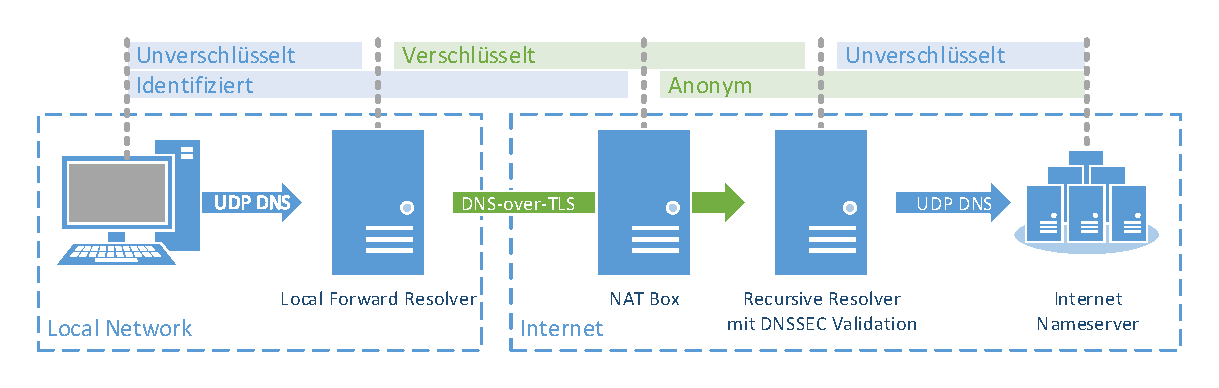
\includegraphics[width=\textwidth,trim={5mm 5mm 5mm 5mm},clip]{Impl_Architecture}
    \caption{Darstellung des schematischen Kommunikationswegs des Test-Aufbaus.}
    \label{img:impl-architecture}
\end{figure}

Um die Privacy der lokalen Clients und damit der Nutzenden zu wahren, wurde der Aufbau nach einem einfachen Grundkonzept entworfen: Entschlüsselte DNS-Nachrichten dürfen nur auf direkt kontrollierten Komponenten mit der externen Internet-Adresse verknüpfbar sein. Dadurch wird verhindert, dass Betreiber der Transportnetzwerke oder der nachgeordneten DNS-Komponenten private Daten mit den persönlichen Identitäten verknüpfen können.

Des weiteren wird durch DoT jede Form von Sniffing und Spoofing Attacken unmöglich gemacht. Da der Forwarding-Resolver selbst keine normalen DNS Anfragen von außerhalb des lokalen Netzwerks annimmt, ist der Resolver gegen DNS DoS Attacken durch externe Angreifer geschützt. Die \ac{DNSSEC} Validierung erfolgt je nach Implementation am lokalen Forward-Resolver oder am Public-Recursive-Resolver. Es ist damit selbst im Falle einer erfolgreichen Cache-Poisoning Attacke auf den Public Resolver nicht möglich, RRs zu kompromittieren, die durch \ac{DNSSEC} Signaturen geschützt sind.

\section{Aufbau}
\label{sec:architecture}
Zu Validierung des Entwurfs wurde ein einfacher Test-Aufbau umgesetzt. Dieser verwendet Windows 10\footnote{Microsoft Windows Version 1803 (Build 17134.285)} als Test-Client-Betriebssystem und Fedora 28\footnote{Linux 4.17.19-200.fc28.x86\_64} als Betriebssystem des lokalen Resolvers. Der Local-Resolver selbst wurden zwecks Vergleichbarkeit mit zwei verschiedenen Software-Paketen umgesetzt: Unbound\footnote{Version 1.7.3 (kompiliert mit OpenSSL 1.1.0h-fips)} und Knot-Resolver\footnote{Version 2.4.1}. Als Trusted-Public-Resolver wurde das Quad9-Projekt gewählt, da es DoT anbietet und einer zu befürwortende Privacy-Policy \cite{Quad9Privacy} folgt. Darüber hinaus werden Domänen, die in Zusammenhang mit Schadsoftware stehen, vom Quad9-Resolver automatisch geblockt. Dieses Feature kann zwar als Zensur verstanden werden, durch die aktuelle Bedrohung durch DNS unterstützte Malware \cite{Alcoy2017} und die strikt auf ``Phishing, Malware, and Exploit-Kits'' konzentrierte Sperrliste \cite{Quad9FAQ} kann die Bedrohung durch Zensur der durch Malware vorübergehend untergeordnet werden.   
\begin{wrapfigure}{r}{0.5\textwidth}
    \begin{center}
    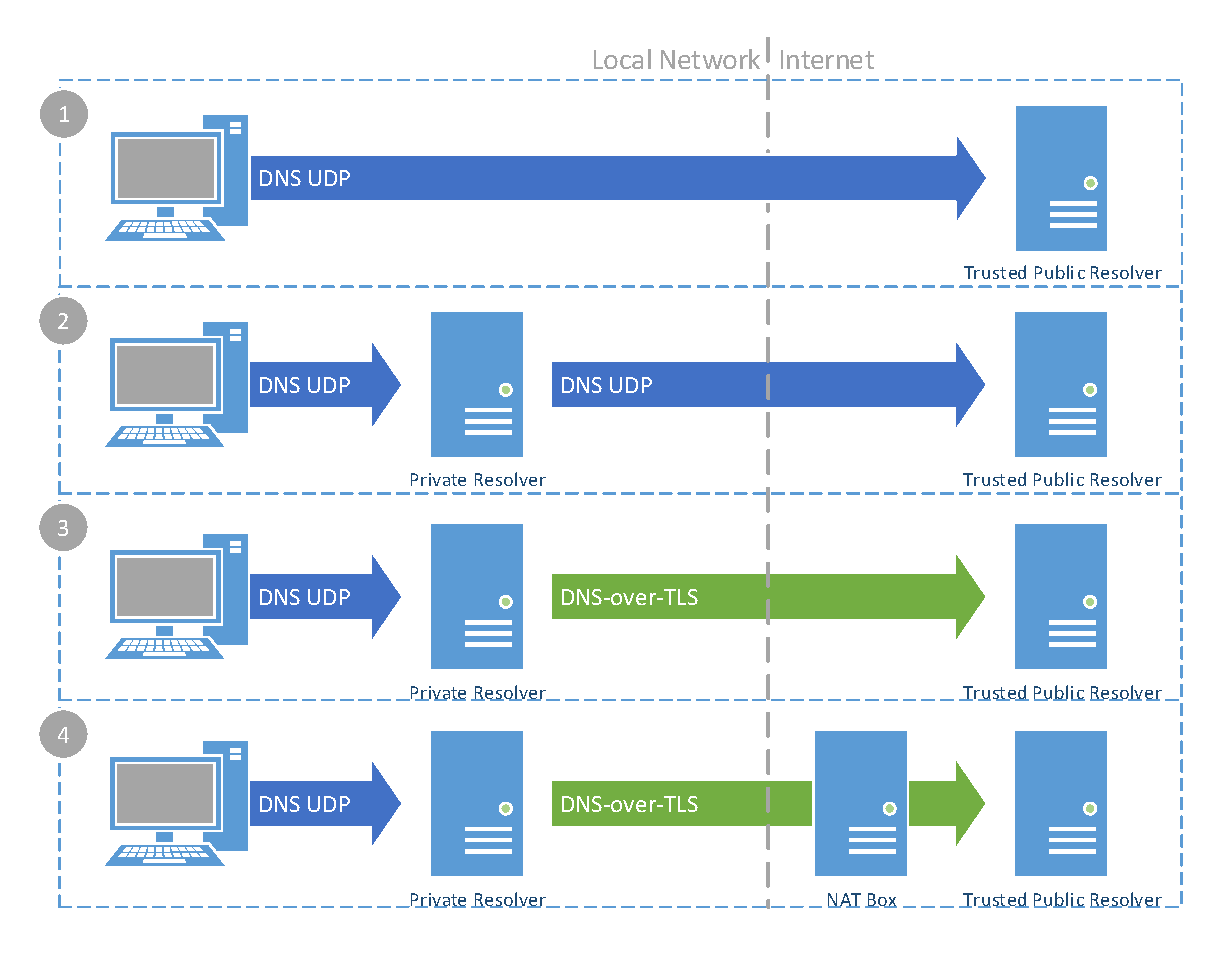
\includegraphics[width=0.48\textwidth,trim={5mm 8mm 5mm 8mm},clip]{Impl_Scenarios}
    \end{center}
    \caption{Darstellung der getesteten Szenarien}
    \label{img:impl-scenarios}
\end{wrapfigure}

Wie in Abbildung \ref{img:impl-scenarios} dargestellt wurden für den Performance- und Funktions-Test vier Szenarien gewählt. Nur Szenario 4 erfüllt alle beschriebenen Schutzmechanismen. Szenario 3 verletzt lediglich die Anonymität gegenüber dem Public-Resolver. Geht man von einem vertrauenswürdigen Anbieter dieses Resolvers aus, kann auf die Anonymisierung über den NAT-Server verzichtet werden. Wie man sieht, wird in jedem Fall von einem sicheren lokalen Netzwerk ausgegangen. Mögliche Lösungen bei unsicheren Netzwerken werden in Kapitel \ref{chap:conclusion} diskutiert. 

\paragraph{Public-Resolver über UDP (1)}
Durch die direkte Verbindung zwischen Stub-Resolver und Public Resolver wird auf jegliche Vertraulichkeit der Übertragung verzichtet, da der in Windows integrierte Stub-Resolver keine Form der Verschlüsselung unterstützt. Abgesehen davon, ergibt sich durch die minimale Anzahl an Zwischenstellen eine optimale Latenzzeit, die sich positiv auf die gesamte Performance auswirkt.

\paragraph{Lokalen Forwarding-Resolver über UDP (2)}
In diesem Fall wird ein Forwarding-Resolver im lokalen Netzwerk installiert. Da dieser das klassische DNS-Netzwerkprotokoll zur Kommunikation mit dem Recursive-Resolver verwendet, ergibt sich noch kein Schutz der Vertraulichkeit. Mit einer restriktiven Konfiguration und verschiedenen, von der Implementation abhängigen, Sicherheitsfeatures können jedoch gewisse Arten von Spoofing-Attacken ausgeschlossen werden. Befindet sich eine Firewall an der Netzwerkkante so kann diese, durch den Einsatz eines lokalen Resolvers, sehr restriktiv eingestellt werden. Dies verhindert direkte Angriffe auf Stub-Resolver von extern. Ein weiterer Vorteil besteht beim Einsatz von ``Knot-Resolver'' da dieser bestimmte DNS Rebinding Attacken (siehe \ref{sec:attack-dnsrebind}) abwehren kann, indem er interne IP-Adressen in Antworten verbietet \cite{KnotResolverDocRebinding}.

\paragraph{Lokaler Forwarding-Resolver mit DoT (3)}
Wird die Verbindung zum Recursive-Resolver durch ein Verschlüsselungsprotokoll wie DoT (siehe \ref{sec:tec-dot}) geschützt, ergibt sich ein klarer Vorteil: Es besteht eine sichere Verbindung zwischen dem Forwarding- und Recursive-Resolver, was Sniffing-, Spoofing-, sowie MITM-Attacken auf diesem Wege ausschließt. Durch den Einsatz von verbindungsorientierten Protokollen und Verschlüsselung werden jedoch der steigende Ressourcenverbrauch und höhere Latenzzeiten merkbar.

\paragraph{Lokaler Forwarding-Resolver mit DoT und NAT (4)}
Fügt man dem Aufbau einen NAT-Server (siehe \ref{sec:tec-nat}) hinzu, erhält man den Vorteil der Anonymität gegenüber dem Recursive-Resolver. Da dies der einzige Vorteil des Aufbaus darstellt, ist die dadurch einhergehende Erhöhung der Latenzzeit gegen den Schutzbedarf abzuwägen.

\section{Tests und Messungen}
\label{sec:measurements}
Die Kontrolle der unter \ref{sec:architecture} beschriebenen Varianten wurde mithilfe der Programme dig\footnote{Auf Ubuntu Subsystem for Windows10; DiG 9.10.3-P4-Ubuntu} sowie ``DNS Benchmark''\footnote{von Steve Gibson Version 1.3.6668.0} durchgeführt. Gemessen wird die gesamte benötigte Umlaufzeit (Round-Trip-Time; RTT) 100 ungecachter, zufälliger Einträge. Die gewählten Konfigurationen der DNS-Server sind in \nameref{chap:appA} zu finden und wurden nach den offiziellen Dokumentationen und darin enthaltenen Sicherheitsempfehlungen erstellt. Als ``Hardware'' wurden 3 virtuelle Maschinen (1 vCPU, 1GB RAM) auf einem vom Test-Client unabhängigen Host genutzt. Um eine optimale Vergleichbarkeit der einzelnen Varianten zu erreichen wurden die Tests der Performance von einem Test-Client auf die 3 Server simultan durchgeführt. Dabei wurden in 2 unabhängigen Läufen alle unterschiedlichen Varianten einer Software getestet. In einem dritten Lauf wurde die direkte Performance von 25 offener DNS-Resolvern (siehe \ref{chap:appB}) getestet und die 10 besten zur Errechnung der direkten Vergleichswerte herangezogen. Für die Auswertungen wurden immer nur Werte von ungecachten Einträgen herangezogen, da nur diese eine Kommunikation mit dem Recursive-Resolver verlangen. Die Ergebnisse der Tests sind unter Kapitel \ref{chap:results} angeführt. 

